%!TEX root = ../main.tex
\chapter{État de l'art}
Deux sujets principaux seront abordés dans ce mémoire : la sécurisation d'une chaîne de production DevOps et la 
gestion opérationnelle de la sécurité d'une infrastructure \ac{K8S}.

Il me semble donc pertinent de présenter les risques de sécurité associés à ces deux sujets indépendamment afin de 
pouvoir mieux les définir et éventuellement démonter un certain recoupement avec d'autres problématiques de sécurité 
informatique. 


\section{Évaluation des risques de sécurité}

\subsection{Les risques du Pipeline DevOps}
Dans la méthodologie DevOps, le \emph{Pipeline} est un concept hybride regroupant des notions théoriques et un socle 
technique utilisés dans le cadre d'un développement logiciel. Ainsi, l'utilisation du terme \emph{Pipeline} fait aussi 
bien référence au \ac{SDLC} \autocite[Ch.\ 6]{devops_for_dummies_freeman_forsgren_2019}, aux standards de développement
\autocite[Ch.\ 9]{devops_for_dummies_freeman_forsgren_2019},qu'au processus de qualification et validation, ou bien même
à l'ensemble des outils et services utilisés par les équipes de développement. 
\newline Il s'agit donc d'un élément centrale dans la chaîne de production DevOps: tout problème impactant un élément du 
\emph{Pipeline} aura des répercussions sur les autre et risque ainsi de mettre en péril les opérations de développement.

Nous pouvons donc nous poser la question de la nature des risques portés par le \emph{Pipeline}; et tout particulièrement
ceux portant sur l'aspect sécurisation informatique.
\newline Pour cela, nous allons utiliser comme support un \ac{SDLC} DevOps afin de mieux cibler les 
problématiques de sécurité à chaque étape d'un projet.

\vspace{0.5em}
\begin{figure}[h]
    \centering
    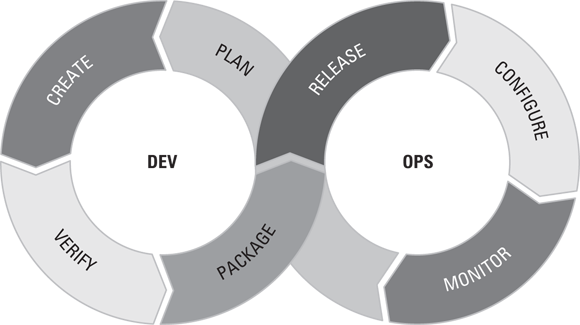
\includegraphics[width=0.5\linewidth]{resources/img/devops_lifecycle.png}
    \captionsource{Représentation du cycle de vie d'un projet DevOps}{DevOps for Dummies, Figure 6-1}
    \label{fig:devops-lifecycle}
\end{figure}
\newpage

Après une rapide analyse, voici les principaux risque qui se présente à nous :
\begin{multicols}{2}
    \begin{enumerate}
        \item Plan :
        \begin{itemize}
            \item Intégration d'une technologie vulnérable ou non maintenue
            \item Non-intégration de correctifs pour une vulnérabilité remontée
        \end{itemize}
        \item Create :
        \begin{itemize}
            \item Développement de code faillible
            \item Mauvaise configuration du framework ou dépendances
        \end{itemize}
        \item Verify :
        \begin{itemize}
            \item Jeux de test incomplets
            \item Absence d'audit de sécurité applicative
        \end{itemize}
        \item Package :
        \begin{itemize}
            \item Utilisation d'un OS ou paquets vulnérables
            \columnbreak
            \item Erreur de configuration du conteneur
            \item Erreur de configuration des services
        \end{itemize}
        \item Release :
        \begin{itemize}
            \item Mauvaise gestion des versions de conteneurs
            \item Erreur de configuration du script de build
        \end{itemize}
        \item Configure :
        \begin{itemize}
            \item Mauvaise gestion des secrets
            \item Erreur de configuration des déploiements
        \end{itemize}
        \item Monitor :
        \begin{itemize}
            \item Absence ou trop faible collecte de log (application et conteneur)
        \end{itemize}
    \end{enumerate}
\end{multicols}

On constate donc qu'une majorité des risques protés par le \emph{Pipeline} DevOps sont lié à des erreurs commises lors
du développement. Il s'agira donc d'un point d'attention dans la recherche de solutions.

\subsection{Les risques d'un cluster Kubernetes}
De par sa nature, l'orchestrateur \ac{K8S} et les nœuds qui constituent le cluster agissent comme une couche 
d'abstraction entre l'infrastructure du Cloud Provider et les conteneurs (aussi appelés \emph{Pods}) qu'il héberge.
\newline Il est cependant important de noter que quelques problématique de sécurité (\eg Réseau, accès API, chiffrement 
du traffic \emph{etcd}, \dots) sont tout de même à addresser. C'est en tout cas ce que recommande la documentation 
officiel de \ac{K8S}\autocite{k8s_security_2021}.

Nous nous retrouvons donc avec les risques propres au cluster \ac{K8S} qui, dans un certain sens, partage des similitudes
avec les risques protés par des infrastructure virtualisés classique : Gestion du \ac{RBAC} et de l'authentification, 
gestion des secrets, qualité de service, etc..

Cependant, le fonctionnement d'un conteneur est différent d'une machine virtuelle : le kernel est partagé entre l'hôte et
le conteneur. De nouveaux risques apparaissent d'isolation d'environnements d'execution et d'accès à des ressources 
sensible apparaissent donc. 

\newpage

\section{Recherche de solutions}

Ayant identifié les risques encourus par notre Pipeline DevOps et l'infrastructure Kubernetes associée,
nous pouvons maintenant nous intéresser aux solutions permettant leurs réductions.

Pour cela nous allons utiliser comme support la méthodologie décrite dans le \citetitle{samm_v2.0_owasp_project_2021}
\autocite{samm_v2.0_owasp_project_2021}
de l'\citeauthor{samm_v2.0_owasp_project_2021}. Cette méthodologie, mit à jours en 
\citedate{samm_v2.0_owasp_project_2021}, fait office de référence pour l'analyse et l'amélioration de la sécurité des 
logiciels développés en entreprise.
\newline Elle est particulièrement recommandé dans le cadre de développement Agiles et / ou \linebreak DevOps.

\subsection{Le modèle de référence}

Le \ac{SAMM} est, comme son nom l'indique, un modèle permettant de quantifier le niveau de maturité d'un processus de 
développement logiciel sur le plan de la sécurité informatique. 

Cette quantification est réalisée sur la base de différentes pratiques de sécurité chacune regroupés dans des fonctions 
métier et notés sur une échelle de trois points avec en point initial zéro implicite. 
\newline Ces pratiques de sécurité dispose elles même de deux activités permettant de qualifier le niveau de maturité 
d'une entreprises sur les principaux thèmes associée à la pratique.

Le \ac{SAMM} peut donc être représenté de la manière suivante :

\begin{figure}[h]
    \centering
    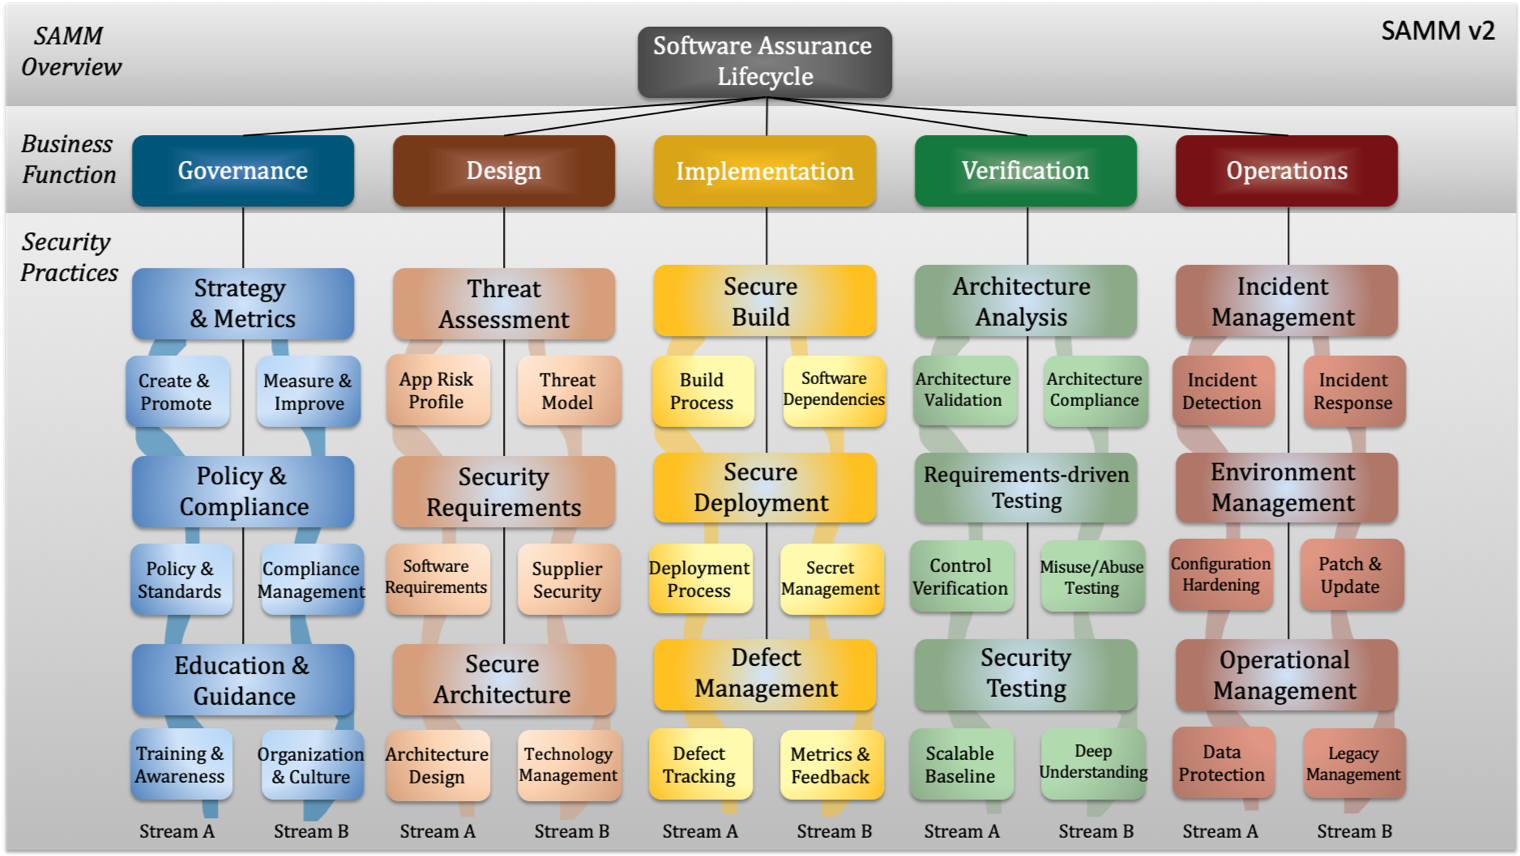
\includegraphics[width=1\linewidth]{resources/img/Samm_v2.png}
    \captionsource{Modèle SAMM v2}{Release note v2, \href{https://owaspsamm.org/release-notes-v2/}{OWASPSAMM.org}}
    \label{fig:samm-rep}
\end{figure}

\newpage

L'échelle de quantification quant à elle est défine de la manière suivante : 
\setlist[enumerate,1]{start=0}
\begin{enumerate}
    \item Niveau initial, aucune mesure de sécurité n'est appliqué.
    \item Niveau de compréhension basique de problématiques de sécurité et application de mesure ad hoc.
    \item Niveau avancé d'application des mesures de prévention avec constatation de l'efficacité ces dernières.
    \item Niveau de maîtrise complète des pratiques de sécurité à l'échelle de l'organisation.
\end{enumerate}
\setlist[enumerate,1]{start=1}
On considérera dans cette mission que le second niveau est un prérequis à la validation des pratiques de sécurité.
Le dernier niveau constitue quant à lui l'objectif à atteindre.

\subsection{Gouvernance}

La fonction \emph{Gouvernance}, telle que présentée dans le modèle \ac{SAMM}, représente le point de départ de la 
mise en œuvre de la sécurité informatique dans le cadre de développement. C'est en effet sur la base des 
trois pratiques de sécurité associés (\emph{Stratégie \& Métriques}, \emph{Politiquer \& Conformité}, 
\emph{Formation \& Conseils}) que seront issue l'ensemble des actions techniques et organisationnels des autres
fonctions métier.

La \emph{Gouvernance} de la sécurité des développements est un sujet déjà encré dans la philosophie du Groupe JCDecaux.
Il dispose déjà d'un niveau de maturité avancé grâce à la mise en place de politiques de sécurité dédiées au 
applications et leur développement; à la formation et intégration d'interlocuteurs sensibilisé aux risques de sécurité;
de même que la mise en place de \ac{KPI} permettant la mesure et l'amélioration de l'efficacité de la stratégie.
\newline Cette stratégie, adoptant les principes de la sécurité par la conception (Security By Design) a par ailleurs 
fait  l'objet d'une présentation\autocite{devopsrex_denis_2019} lors du \href{https://2019.devopsrex.fr/}{DevOpsREX 219} 
par Joy-Alexandra Denis, ex-RSSI du Groupe JCDecaux et maintenant RSSI de la filiale France du Groupe Ikea.

Cependant, et contrairement aux préconisations du \ac{NIST}\autocite*{app_cont_sec_nist_2017}, le Groupe ne dispose pas
d'une politique de sécurité dédié aux technologies de conteneurisation d'application et d'hébergement connexe. 

De même, bien que l'on observe une forte sensibilisation aux problématiques de sécurité des responsables produit / 
projet, on constate que les populations de développeurs ne disposent pas d'un accompagnement spécifique et
institutionnalise au niveau du groupe sur ces \linebreak problématiques.

Ainsi, le \ac{SAFECODE} recommande la mise en place d'une formation continue des équipes de développement aux techniques
de sécurisation de code et au développement sécurisé dans son rapport \citetitle{six_pillarss_devsecops_safecode_2020} de 
\citedate{six_pillarss_devsecops_safecode_2020}.

\newpage

\subsection{Conception}

Si l'on considère que la \emph{Gouvernance} constitue les fondations d'un développement applicatif sécurisé, la 
conception et l'imagination de son architecture représente quant à elle l'ossature de cette dernière : une faiblesse dans 
la conception pourrait entraîner la compromission globale de l'application. 
\newline Afin de prévenir ces risques, le modèle \ac{SAMM} identifie trois axes de sécurisation : l'évaluation des risques, 
la définition de prérequis de sécurité et la sécurisation de l'architecture.

Depuis 2019, toutes les applications produites au sein du Groupe JCDecaux font l'objet d'une analyse de risque 
(voir annexe \ref{appendix:securitybydesign}) par les équipes de développement dès l'étude de faisabilité. 
Cette analyse de risque et les prérequis de sécurité associé seront ensuite soumis à validation par l'équipe \ac{SSI} 
qui émettra des recommandations si cela est nécessaire.

Si certain prérequis de sécurité sont directement dépendent directement de l'application développée, il est important 
de noter que la \ac{SAMM} et le \ac{SAFECODE}\autocite[p. 15]{fundamental_pract_sec_soft_safecode_2018} recommandent la 
mise à disposition des équipes de prérequis génériques pour les développement.
\newline Dans le cas du Groupe JCDecaux, ces recommandations sont présenté sous la forme de onze \emph{Golden Rules}
rédigés en anglais et disponible pour toutes les équipes de développement du Groupe.

Enfin, il conseillé de définir un set d'architectures applicative standard pour les développement. Cela peut prendre la 
forme d'une architecture Type ou d'une configuration modèle d'un framework .

\subsection{Implémentation}
L'implémentation, étape la plus chronophage dans un projet de développement, représente la principale activité des 
développeurs. C'est durant cette étape que ces derniers produisent le code source et ressources qui constituerons 
l'application une fois compilée.

Afin de disposer d'une base commune de développement et de process, ces même développeurs mettent en œuvre divers outils
à unifier les environnements et d'automatiser le plus d'actions. On retrouve donc des outils de versionnage de code, 
d'execution de tests automatiques ou bien encore de compilation et livraison automatique d'images\footnote{Ces outils de \ac{VCS}, 
\ac{CI}, \ac{CD} constituent dans les faits la base technique du Pipeline DevOps.}.

Ces outils étant performant et versatiles, la méthodologie \ac{SAMM} nous propose de les exploiter et ou complémenter 
afin de réaliser des opération d'évaluation de sécurité.
\newline Ainsi en intégrant des analyseurs de dépendances et en rajoutant des règles dans les profils d'évaluation de 
qualité de code, il est possible de drastiquement réduire le nombre de vulnérabilité d'un programme.
Dans le cas où l'intégration de ses règles seraient trop coûteuses ou impossible, l'exploitation d'outils dédiés est 
envisageable. Ces outils sont des \ac{SAST}. 

Autre point important lors de l'implémentation, une gestion appropriée des configuration et des secrets est requise pour
toute conception d'application conteneurisée. En effet, il est primordiale de stocker ses configurations et secrets dans
un référentiel unique et auditable. Il en va de même pour les images compilée.

Cette centralisation des ressources par type permettra un meilleur suivi des défauts et par la suite la mise en place 
de \ac{KPI}. Ces \ac{KPI} pourront servir à l'évaluation des performances de sécurité des application, mais aussi au 
ciblage des équipes nécessitant d'être accompagnée sur ce sujet.
\newline L'objectif final étant de pouvoir faire évoluer continuellement la gestion de la sécurité des applications grâce
à ces \ac{KPI}.

\subsection{Vérification}
Partie intégrante du développement applicatif, la phase de validation vise à tester toutes les fonctionnalités de 
l'application pour découvrir d'éventuellement dysfonctionnements.
\newline Dans le cadre de la méthodologie \ac{SAMM}, cette étape se présente sous la forme de trois pratiques de sécurité.

Dans un premier temps, il sera nécessaire de analyser l'architecture de l'application et de son implémentation dans le 
\ac{SI} à la recherche de vulnérabilités connues. Si aucun problème n'est détecté et que les mécanismes de sécurité de 
l'application sont correct, nous pourrons passer à l'étape suivante.
\newline Dans le cas contraire, les développeurs devront revoir leur copie.

Dans un second temps, voir éventuellement en parallèle de l'étape précédente, il sera nécessaire de faire exécuter des 
test d'intégration continue afin de valider le bon comportement de l'application vis à vis de vulnérabilité connue.
Des test de charge et d'attaque sur la logique métier de l'application sont par ailleurs fortement recommandé.
\newline Des solutions de \ac{DAST}  et \ac{IAST} tel que les services \href{https://www.rapid7.com/products/insightappsec/}
{Rapid7 InsightAppSec} et \href{https://www.acunetix.com/}{Acunetix d'Invicti} peuvent donc se montrer fort intéressantes.

Enfin, si et seulement si aucun problème n'a été détecté, alors nous pourrons lancer un audit de sécurité (aussi appelé 
\emph{pentest} pour Penetration Testing). Cet audit devra être réalisé sur une instance d'application iso-production afin
de coller le plus possible à l'intégration finale. Un environnements de d'intégration ou de pré-production est donc le 
plus adapté.

Pour le Groupe JCDecaux, on constate une certaine déviation vis à vis des recommandations de la méthodologie \ac{SAMM}.
Si la validation de l'architecture et les audits de sécurité sont bien réalisés, la portion \ac{DAST} / {IAST} n'est 
quand à elle pas présente.

\subsection{Opérations}
Si jusqu'ici les différentes solutions proposés par la méthodologie \ac{SAMM} et le groupe \ac{SAFECODE} portaient sur
la sécurisation du \emph{Pipeline} DevOps, cette dernière fonction métier se concentrera essentiellement la sécurisation
de l'exploitation de l'application développé, et donc du cluster l'hébergeant.

Le premier aspect de sécurité opérationnelle à addresser portent sur la façon dont un conteneur fonctionne sur le cluster.
Ainsi, il est nécessaire de pouvoir durcir les configuration d'exécutions des pods, soit en fournissant des outils de 
configuration automatique, soit en  appliquant des point de contrôle bloquant lors du déploiements d'un conteneur sur un 
cluster.

Deuxième aspect d'importance, la connaissance des pods en cours d'exécutions sur un cluster ainsi que la connaissance de
leur état de vulnérabilité est primordiale à la sécurisation du cluster. Ainsi, comme pour les infrastructure "classiques",
l'exploitation de scanner de vulnérabilité est une nécessitée pour disposer d'informations suffisante et fiable pour
avoir une gestion appropriée des patchs de sécurité.

De même que le besoin se fait sentir pour les infrastructure virtualisés, la gestion des incidents sur les clusters doit 
être efficace et proactive. Cela sous-entends d'avoir à disposition une procédure décrite de manière exhaustive et connue
par les équipes en lien avec la plateforme.
\newline La premières source d'information pour la gestion d'incidents sera les logs applicatifs et issues du cluster, 
mais ceux-ci peuvent être complémenter par des informations liés à runtime du conteneur. C'est par exemple ce que propose
la solution \href{https://sysdig.com/opensource/falco/}{Falco de sysdig}.

Enfin, une bonne gestion des donnée vas de paire avec la gestion du cycle de vie de l'application.
\newline Toute donnée exploitée par un conteneur doit être d'une utilité légitime et chiffrée dans le cas où elles sont
à caractère sensible.
 

\newpage

\section{Analyse et critique des solutions}